\documentclass[../lab2.tex]{subfiles}

\begin{document}
    In un secondo caso piu' semplice abbiamo coinvolto solo il router e 
    il PC Live Linux.
    Campionando i primi dati abbiamo notato che in seguito alla prima frammentazione
    il firewall del router scartava i pacchetti successivi. Abbiamo provato a cambiare
    la configurazione del firewall dell'interfaccia di rete per permettere la risposta 
    a pacchetti con dimensione maggiore di MTU

    \begin{center}
        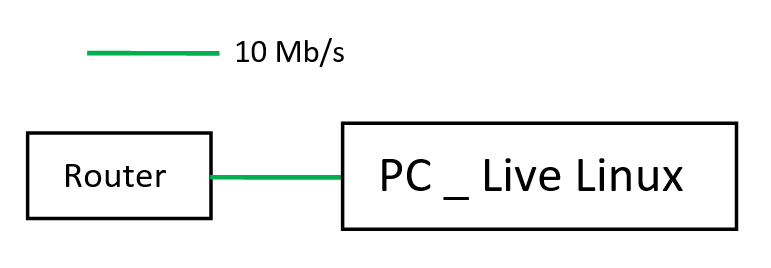
\includegraphics[width=0.3\linewidth]{conf2.png}
    \end{center}
\end{document}